\documentclass{article}
\usepackage{relsize}
\usepackage{lmodern}
\usepackage{textcomp}
\usepackage{graphicx}
\usepackage{hyperref}
\usepackage{listings}
\usepackage[utf8]{inputenc}

\title{The truth about chatbots \\[0.4em]\smaller{}Session n\,°3: The technical stack}
\author{Louise Crépet}
\date{March 2019}

\begin{document}

\maketitle

\textit{Special thanks to Hugo Hache for letting me steal his slides!}

\newpage
\section{The chatbot theory}
The basic principle of a chatbot is the following: trying to understand something, in order to answer something. \\
What’s “understand”? It’s get a message and make sense of it.\\
What’s “answer”? It’s build a response and transmit it.\\
\newline
So we have 4 blocks: get, make sense, built, transmit.\\

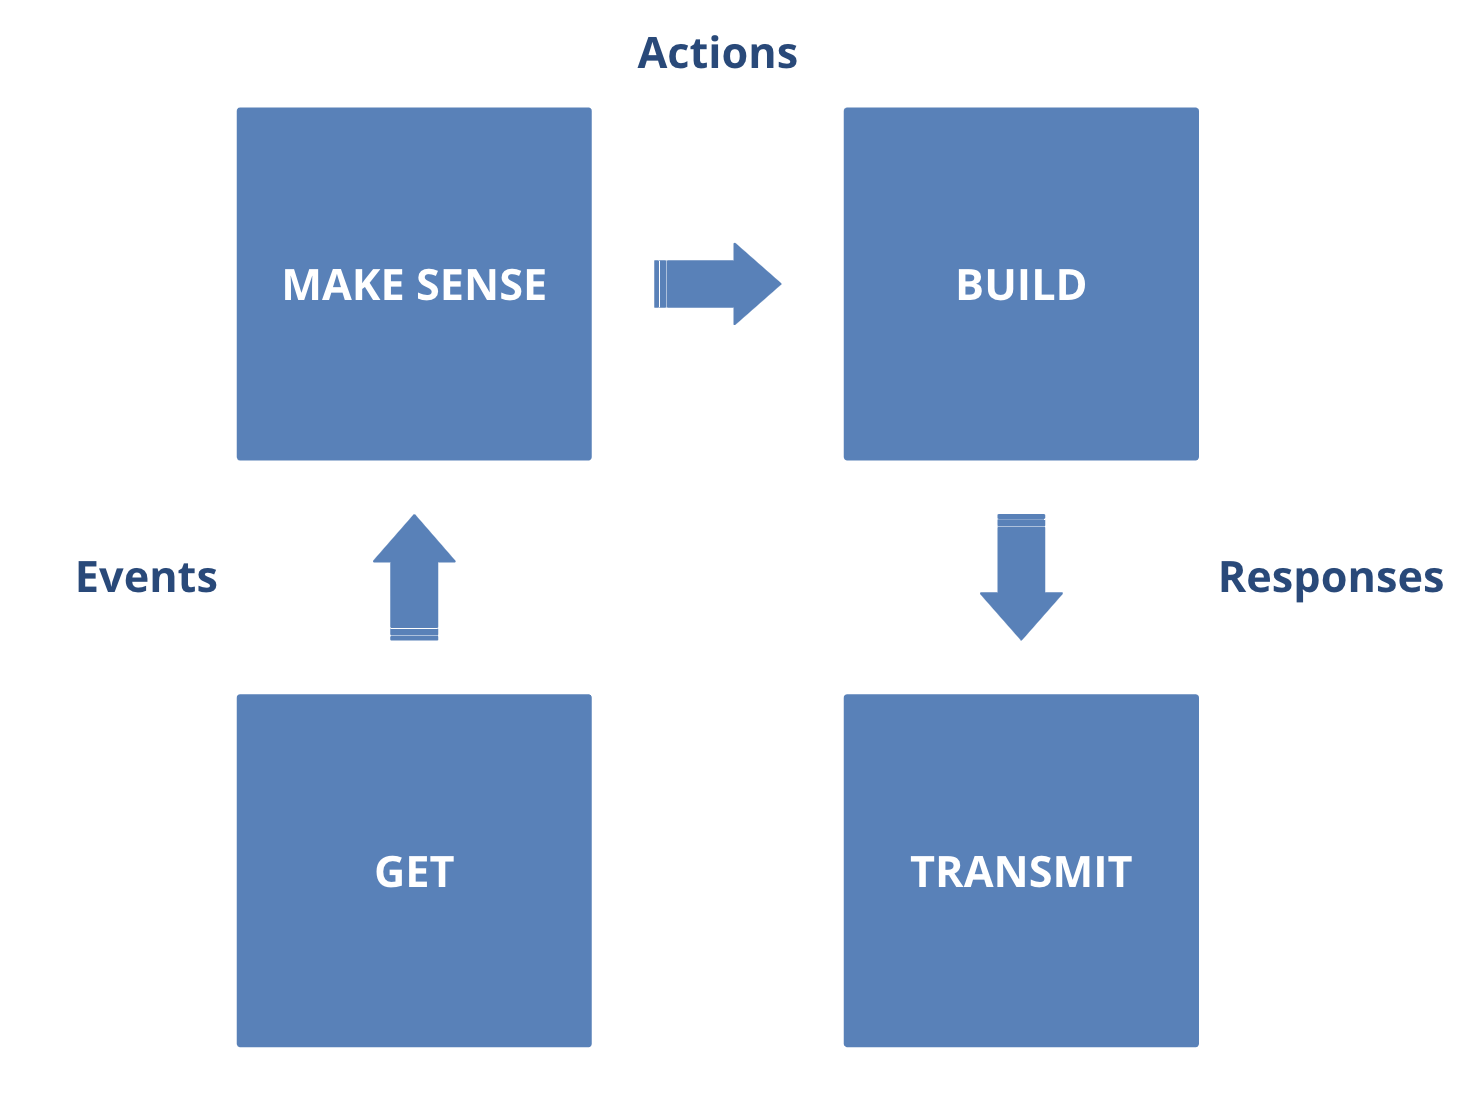
\includegraphics[scale=0.4]{images/chatbot_blocks.png}
\newline
The “get” and “transmit” parts can be handled by the same block: a connector. A connector is basically this: an element which allows the chatbot to:
\begin{itemize}
    \item get an event from a channel 
    \item transmit a response to a channel
\end{itemize}

The “make sense” block can partly be made by a NLP engine. It will transform the text contained in the event into parameters.
If the input is a command, or if the user clicked on a button, the parameters can be extracted by a simple parser. Once the parameters are known, one or more actions can be executed to build the answer.

The “build” block is the job of the “bot” part of the chatbot. After it “made sense” of the input, it will do some actions to build the response.
The term “action” can designate: 
\begin{itemize}
    \item the computation of a value
    \item the call of an external API
    \item the persistence of data
\end{itemize}

All the parties involved in these blocks can be linked like this:

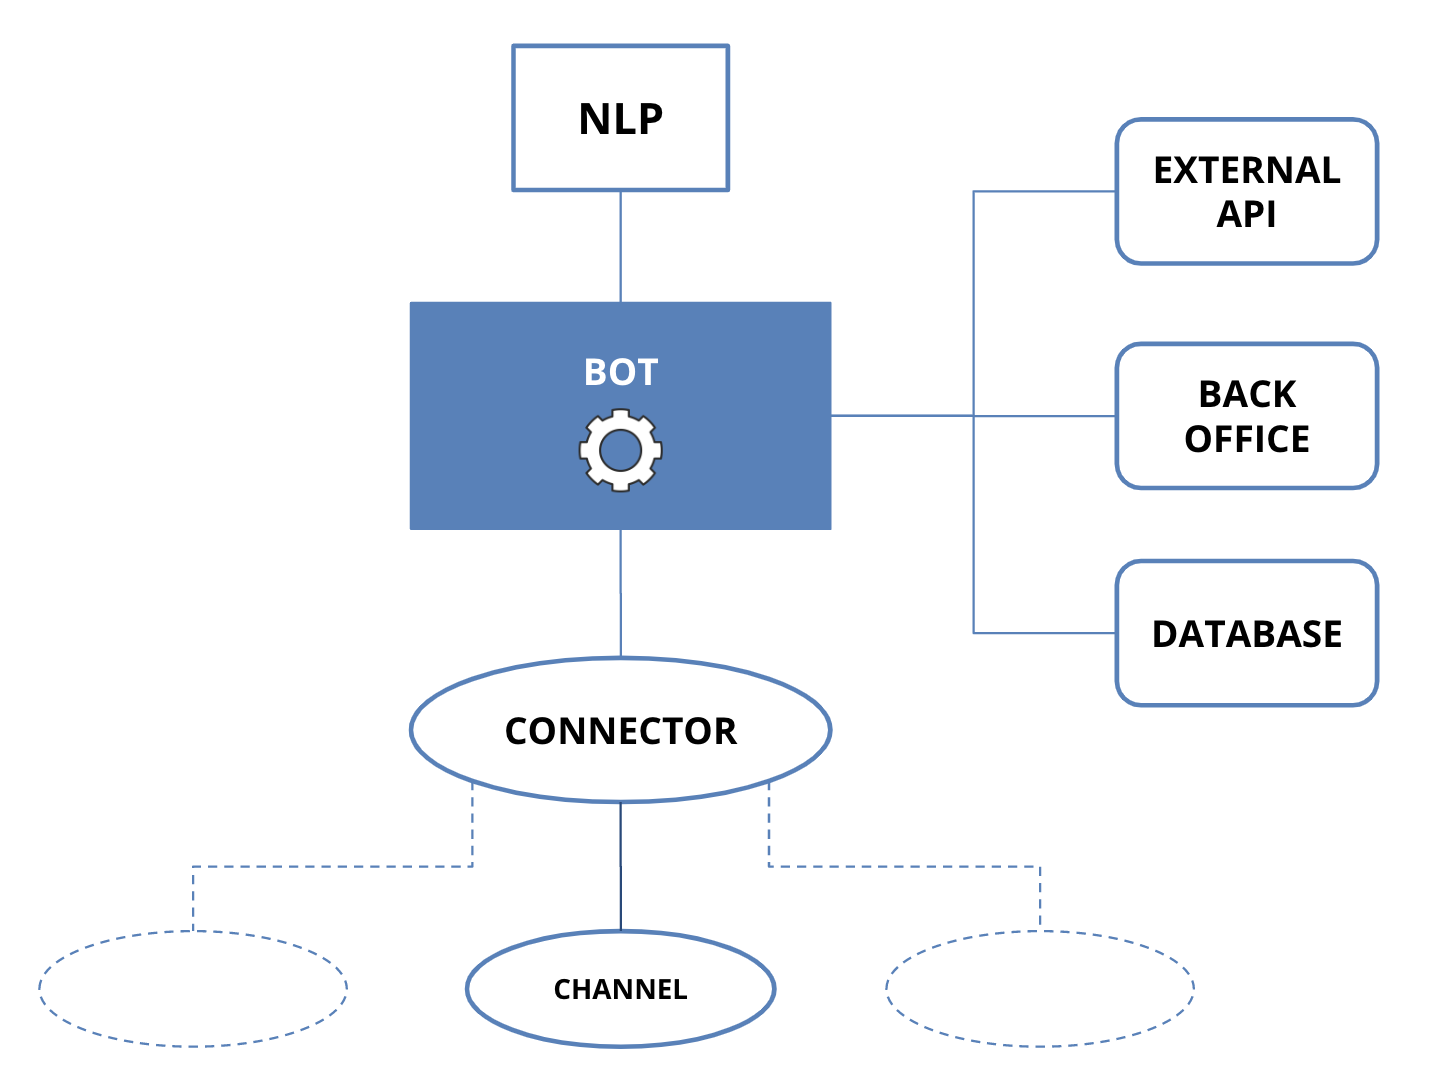
\includegraphics[scale=0.4]{images/chatbot_archi.png}
\newpage
\section{Channels}
How do we make a chatbot available on a channel, like Facebook Messenger?
\newline
\newline
First, some definitions:
\begin{description}
    \item \textbf{Webhook}: method for augmenting or altering the behaviour of a web page, or web application, with custom callbacks.
    \item \textbf{API}: set of clearly defined methods of communication among various components.
    \item \textbf{HTTP}: protocol used to communicate  on the internet.
    \item \textbf{HTTP request}: message sent by a client (something that sends messages) to a server (something that receives messages), using HTTP.\\
\end{description}
Most of the channels allow to use webhooks. The chatbot subscribes to events on the channel administration platform: it creates a webhook. The interesting event is usually "one user sent a message", but the channel can offer other, like "one user just connected".

Each time one the the events occurs, the channel informs the chatbot. For that, it sends an HTTP request to the chatbot API.

The chatbot can send a response using the channel API.\\
\newline
For example, let's try to set up a chatbot on Facebook Messenger:
\begin{enumerate}
    \item Go to the \href{https://developers.facebook.com/}{developers Facebook console}.
    \item Create a new Facebook page.
    \item Create a new Facebook application.
    \item In the settings page of your application, add a new product: Messenger.
    \item Click on "Messenger" and go to the "Webhooks" section.
    \item Add permissions: messages and messaging\_postbacks.
    \item Add the URL of your chatbot API: it has to return a 200 HTTP status when Facebook Messenger sends a GET request. FB Messenger will send POST requests to this URL to inform the chatbot an event occured.
    \item Select your FB page to link it to your app.
    \item Go to the "Access tokens" section.
    \item Authorize your app on your account (only you will be able to talk to your chatbot,  you have to  submit the chatbot to publish it)
    \item Select your FB page to  generate the token. Your chatbot will  use this token to request the FB Messenger API.
    \item You can search your chatbot on Messenger and talk to it!
\end{enumerate}
\newpage
\section{Clarke}
Clarke is a library developed by FTA. It allows to build chatbots.\\
\newline
Its first role is to be a "connector". It connects the chatbot to different channels. The main advantage is that it makes the chatbot “channel agnostic”: you just have to add the corresponding Clarke UI libraries, and Clarke can handle multiple channels. It takes HTTP requests from external platforms and transforms them into events that the bot can understand. For example, when a user sends a message via FB Messenger, it looks like this:
\begin{lstlisting}
        {
          "entry":[{
            "messaging":[{
              "sender":{ "id":"USER_ID" },    
                "recipient":{ "id":"PAGE_ID" },
                "message":{
                "text":"Hello world!"
              }
            }]
          }]
        }
\end{lstlisting}
But if the message is sent via Slack, it looks like this:
\begin{lstlisting}
        {
          "token":"TOKEN",
          "team_id":"TEAM_ID",
          "team_domain":"team",
          "channel_id":"CHANNEL_ID",
          "channel_name":"channel",
          "user_id":"USER_ID",
          "user_name":"user",
          "text":"Hello world!"
        }

\end{lstlisting}
Clarke generates standard objects from messages: the objects generated from the examples above would both be an event of type text, with a "sender" (USER\_ID) and a "text" ("Hello world!"). There are several types of event: text, button, media...\\
In the same way, Clarke can transform a standard response into a channel response for Facebook Messenger or Slack.\\
For now, we have implemented the Clarke UI libraries for Messenger\footnote{\url{https://github.com/applidium/clarke-messenger}}, Slack and Twilio.\\
\newline
The second role of Clarke is to offer a framework to build chatbots. To achieve that, Clarke has tools: the request builders. They are modules written by the chatbot developer and run one by one. Each request builder can understand one or more type of events and is subscribed to one or more actions. Each one tries to decode a given event until one of them succeeds and obtains a response build by an action.\\
Let's take an example with Jamy: a user clicked on a button.

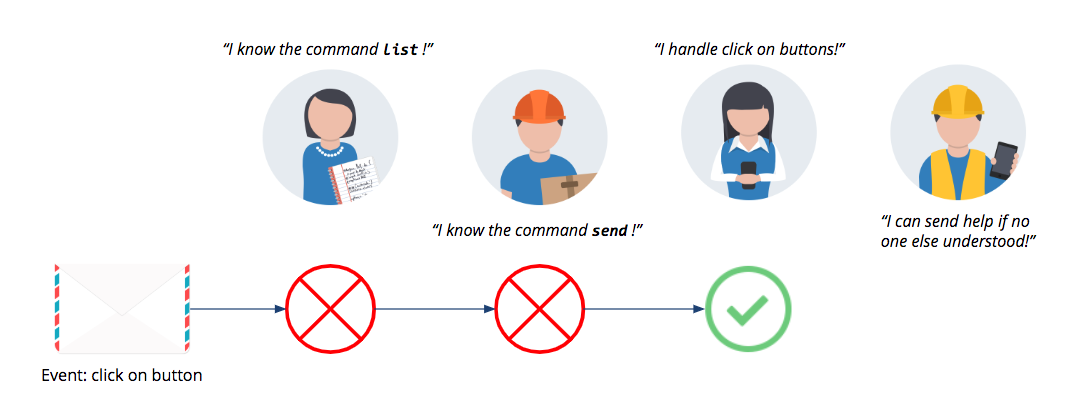
\includegraphics[scale=0.3]{images/jamy_request_builders.png}
\newline
Only the third request builder could handle the event.\\
\newline
Clarke is open-source, you can find it and contribute on Github\footnote{\url{https://github.com/applidium/clarke}}!
\newpage
\section{Natural Language Understanding}
We talk a lot about NLP, but what is it precisely?
\begin{quote}
“Natural language processing (NLP) is [...] concerned with the interactions between computers and human (natural) languages.” \\
(\href{https://en.wikipedia.org/wiki/Natural_language_processing}{Wikipedia})
\end{quote}
According to that definition, automatic translation, text to speech, syntactic parsing, etc are NLP as well. When you want to analyze the sense, you use a sub-domain of NLP:
\begin{quote}
“Natural-language understanding (NLU) [...] is a subtopic of natural-language processing in artificial intelligence that deals with machine reading comprehension.”\\
(\href{https://en.wikipedia.org/wiki/Natural-language_understanding}{Wikipedia})
\end{quote}
There are 3 key concepts in NLU:
\begin{description}
    \item \textbf{Intent}: Mapping between the natural language input and what action should be taken by the software. What does the user want?\\
        \textit{Ex: "\textbf{Launch the quiz} about Heroku level 1."\\
            \hspace*{3pt} \{ "intent": "launch\_quiz" \} }
    \item \textbf{Entities}: Concepts, metadata about intent, used to extract parameters from the natural language input.\\
        \textit{Ex: "Launch the quiz about \textbf{Heroku level 1}."\\
           \hspace*{3pt} \{ "entities": [ "quiz\_name": "heroku", "level": "1" ] \} }
    \item \textbf{Context}: Data from previous inputs. The NLU engine can use them to understand the current input.\\
        \textit{Ex: "Launch the quiz about Heroku. - Which level?"\\
            Input context:\\ \hspace*{8pt} \{ "intent": "launch\_quiz", "entities": [ "quiz\_name": "heroku" ] \} \\
            "I want level 1."\\
            \hspace*{3pt} \{ "intent": "launch\_quiz", "entities": [ "level": "1" ] \}}
\end{description}
Behind that there is an "NLU engine". It's basically a machine learning model which is trained to understand the natural language inputs related to defined intents.\\
How do you train your NLU engine? First, for a given intent, you write a lot of examples. You also can create a dictionary for each entity, to help the engine to recognize them. Then, you  give natural language inputs to the engine, without specifying to which intent they correspond. Finally, you can visualize chat the engine understood or not, and correct it if needed. The machine learning model will then be trained again.\\
\newline
SAP Conversational AI (CAI)\footnote{\url{https://cai.tools.sap}} is a cool platform that provides an NLU engine. You can find an example of a chatbot project on CAI \href{https://cai.tools.sap/lcrepet/quizbot-example}{here}. It contains one custom intent \textit{launch\_quiz} and several "free" intents like \textit{greetings} (the chatbot can understand inputs like "good morning" or "hi dude") or \textit{say-thanks} (the chatbot can understand inputs like "great, thank you" or "cheers"). CAI offers these intents to avoid you to have to train your chatbot for small-talk.\\
CAI can be used as connector too. It also provides an interface to build a chatbot by chaining intents.
\end{document}
